%!TEX root = ../../common/main.tex

\section{CPV measurement}
\label{sec:measurement_of_sin2beta:cpv_measurement}

Utilising the likelihood model presented in
\cref{sec:measurement_of_sin2beta:likelihood_fit} an \acf{uEML} fit is performed
to the nominal data set (\cf
\cref{sec:measurement_of_sin2beta:data_preparation:datasamples}).  The
\MinuitTwo algorithm implemented in the \RooFit (v3.60) framework from \ROOT
v5.34/18 is used to minimise the negative log-likelihood function with the
\emph{minimize} routine and \emph{strategy 2}. \Minos is used for the estimation
of the (asymmetric) parameter errors.

% ------------------------------------------------------------------------------
\subsection{Constrained parameters}
\label{sec:measurement_of_sin2beta:cpv_measurement:constrained_parameters}

Several parameters are incorporated as external inputs. These parameters are
constrained using a Gaussian \PDF with the mean value fixed to the parameter's
value and the Gaussian's width to the uncertainty.
\Cref{tab:measurement_of_sin2beta:cpv_measurement:constrained_parameters} lists
the constrained parameters as well as the source of the value and its
uncertainty employed in the fit.

Individual production asymmetry values are used for the \catOO and \catOT
subsamples. Using the recent \LHCb measurement \cite{Aaij:2014bba} of the
production asymmetry as a function of the \acf{pT} and the \acf{pseudorapidity}
the per-\pT-\pseudorapidity-bin signal fractions $\varepsilon_i =
\sfrac{f_i}{\sum_i f_i}$ of the nominal dataset are determined to calculate a
weighted average of the production asymmetries
%
\begin{equation}
  A_P = \sum_i \varepsilon_i A_{P,i}\eqcm
\end{equation}
where $f_i$ is the number of signal candidates per bin and $A_{P,i}$ the
measured production asymmetry in bin $i$ taken from Ref.~\cite{Aaij:2014bba}.
This yields
%
\begin{equation}
  \begin{split}
    A_P^{\catOO} &= -0.0108 \pm 0.0052 \statp \pm 0.0014 \systp \eqcm \\
    A_P^{\catOT} &= -0.0104 \pm 0.0051 \statp \pm 0.0014 \systp \eqpd \\
  \end{split}
\end{equation}
%
As the measurement has been performed on $\SI{7}{\TeV}$ data only, the numbers for
$A_P^{11}$ and $A_P^{12}$ are highly correlated. We therefore
constraint $A_P^{11}$ in the fit and model $A_P^{12} = A_P^{11} +
\Delta A_P$ with $\Delta A_P = 0.0004 \pm 0.0018 \systp$, where
the systematic uncertainty accounts for the production asymmetry differences
observed for the two data-taking conditions in \LHCb{'s} recent measurement of
the semi-leptonic $\CP$ asymmetry~\cite{Aaij:2014nxa}.
%
\begin{table}
\caption{Parameters that are constrained in the fit.}
\label{tab:measurement_of_sin2beta:cpv_measurement:constrained_parameters}
\centering
\begin{tabular}{lr@{$\,\pm\,$}ll}
  \toprule
  Parameter                        & \multicolumn{2}{l}{Value and uncertainty} & Source \\
  \midrule
  $A_P^{\catOO}$                   & $-0.0108$ & $0.0052$  & \cite{Aaij:2014bba} \\
  $\Delta A_P$                     & $0.0004$  & $0.0018$  & \cite{Aaij:2014bba,Aaij:2014nxa} \\
  $\DMd$ (\si{\planckbar\per\ps})  & $0.510$   & $0.003$   & \cite{Agashe:2014kda} \\
  $\p{0}{\text{\acs*{OS}}}$        & $0.3815$  & $0.0011$  & \cref{eq:flavour_tagging:calibration:os:parameters} \\
  $\p{1}{\text{\acs*{OS}}}$        & $0.978$   & $0.012$   & \cref{eq:flavour_tagging:calibration:os:parameters} \\
  $\deltap{0}{\text{\acs*{OS}}}$   & $0.0148$  & $0.0016$  & \cref{eq:flavour_tagging:calibration:os:asymmetries} \\
  $\deltap{1}{\text{\acs*{OS}}}$   & $0.070$   & $0.018$   & \cref{eq:flavour_tagging:calibration:os:asymmetries} \\
  $\p{0}{\text{\acs*{SS}}}$        & $0.4232$  & $0.0029$  & \cref{eq:flavour_tagging:calibration:ss:parameters} \\
  $\p{1}{\text{\acs*{SS}}}$        & $1.011$   & $0.064$   & \cref{eq:flavour_tagging:calibration:ss:parameters} \\
  $\deltap{0}{\text{\acs*{SS}}}$   & $-0.0026$ & $0.0043$  & \cref{eq:flavour_tagging:calibration:ss:parameters} \\
  $\deltap{1}{\text{\acs*{SS}}}$   & $-0.17$   & $0.10$    & \cref{eq:flavour_tagging:calibration:ss:parameters} \\
  \bottomrule
\end{tabular}
\end{table}

% ------------------------------------------------------------------------------
\subsection{Fixed parameters}
\label{sec:measurement_of_sin2beta:cpv_measurement:fixed_parameters}

As mentioned before, various parameters are fixed in the nominal fit. These are
the mass parameters obtained on simulated data
(\cref{sec:measurement_of_sin2beta:cpv_measurement:fixed_parameters:mass}), the
parameters describing the distribution of the decay time error estimates (\cref{
sec:measurement_of_sin2beta:cpv_measurement:fixed_parameters:decay_time_error:sig,sec:measurement_of_sin2beta:cpv_measurement:fixed_parameters:decay_time_error:bkg}), 
the parameters of the cubic spline functions used to model the \OS and
\SSpi mistag estimate distributions (\cref{sec:measurement_of_sin2beta:cpv_measurement:fixed_parameters:eta:sig:os,sec:measurement_of_sin2beta:cpv_measurement:fixed_parameters:eta:bkg:os,sec:measurement_of_sin2beta:cpv_measurement:fixed_parameters:eta:sig:ss,sec:measurement_of_sin2beta:cpv_measurement:fixed_parameters:eta:bkg:ss}), 
the calibration parameters of the decay time resolution model (\cref{sec:measurement_of_sin2beta:cpv_measurement:fixed_parameters:decay_time_resolution}) 
and the parameters of the cubic spline functions utilised to parametrise
the shape of the lower decay time acceptance (\cref{sec:measurement_of_sin2beta:cpv_measurement:fixed_parameters:acc:au,sec:measurement_of_sin2beta:cpv_measurement:fixed_parameters:acc:eb})
%
\begin{table}
\caption{Fixed mass parameters.}
\label{sec:measurement_of_sin2beta:cpv_measurement:fixed_parameters:mass}
\centering
\begin{tabular}{lr@{$\,\pm\,$}l}
  \toprule
  Parameter                     & \multicolumn{2}{c}{Fixed Value} \\
  \midrule
  $\alpha_{1,m}^\text{\catDD}$      & \multicolumn{2}{c}{$2.28$}\\
  $\alpha_{1,m}^\text{\catLL}$      & \multicolumn{2}{c}{$2.1$}\\
  $\alpha_{2,m}^\text{\catDD}$      & \multicolumn{2}{c}{$2.08$}\\
  $\alpha_{2,m}^\text{\catLL}$      & \multicolumn{2}{c}{$2.43$}\\
  $\lambda_m^\text{\catDD}$         & \multicolumn{2}{c}{$-2.8$}\\
  $\lambda_m^\text{\catLL}$         & \multicolumn{2}{c}{$-3.6$}\\
  $\zeta_m^\text{\catDD}$           & \multicolumn{2}{c}{$0.0$}\\
  $\zeta_m^\text{\catLL}$           & \multicolumn{2}{c}{$0.0$}\\
  $n_1^\text{\catDD}$               & \multicolumn{2}{c}{$3.18$}\\
  $n_1^\text{\catLL}$               & \multicolumn{2}{c}{$3.2$}\\
  $n_2^\text{\catDD}$               & \multicolumn{2}{c}{$6.8$}\\
  $n_2^\text{\catLL}$               & \multicolumn{2}{c}{$4.1$}\\
  \bottomrule
\end{tabular}
\end{table}
%
\begin{table}
\caption{Fixed signal decay time error parameters.}
\label{sec:measurement_of_sin2beta:cpv_measurement:fixed_parameters:decay_time_error:sig}
\centering
\begin{tabular}{llr@{$\,\pm\,$}l}
  \toprule
  \multicolumn{2}{c}{Parameter}              & \multicolumn{2}{c}{Fixed Value} \\
  \midrule
  $f_{\sigma_t}^\text{\catDD,\catOS,\catAU}$ &                       & \multicolumn{2}{c}{$0.069461$}\\
  $f_{\sigma_t}^\text{\catDD,\catOS,\catEB}$ &                       & \multicolumn{2}{c}{$0.09431$}\\
  $f_{\sigma_t}^\text{\catDD,\catSS}$        &                       & \multicolumn{2}{c}{$0.088404$}\\
  $f_{\sigma_t}^\text{\catLL,\catOS}$        &                       & \multicolumn{2}{c}{$0.55165$}\\
  $M_1^\text{\catDD,\catOS,\catAU}$          & ($\si{\pico\second}$) & \multicolumn{2}{c}{$0.037506$}\\
  $M_1^\text{\catDD,\catOS,\catEB}$          & ($\si{\pico\second}$) & \multicolumn{2}{c}{$0.034481$}\\
  $M_1^\text{\catDD,\catSS}$                 & ($\si{\pico\second}$) & \multicolumn{2}{c}{$0.032577$}\\
  $M_2^\text{\catDD,\catOS,\catAU}$          & ($\si{\pico\second}$) & \multicolumn{2}{c}{$0.077666$}\\
  $M_2^\text{\catDD,\catOS,\catEB}$          & ($\si{\pico\second}$) & \multicolumn{2}{c}{$0.072158$}\\
  $M_2^\text{\catDD,\catSS}$                 & ($\si{\pico\second}$) & \multicolumn{2}{c}{$0.059685$}\\
  $M^\text{\catLL,\catOS}$                   & ($\si{\pico\second}$) & \multicolumn{2}{c}{$0.033253$}\\
  $M^\text{\catLL,\catSS}$                   & ($\si{\pico\second}$) & \multicolumn{2}{c}{$0.029475$}\\
  $k_1^\text{\catDD,\catOS,\catAU}$          &                       & \multicolumn{2}{c}{$0.721$}\\
  $k_1^\text{\catDD,\catOS,\catEB}$          &                       & \multicolumn{2}{c}{$0.73243$}\\
  $k_1^\text{\catDD,\catSS}$                 &                       & \multicolumn{2}{c}{$0.72851$}\\
  $k_1^\text{\catLL,\catOS}$                 &                       & \multicolumn{2}{c}{$0.80445$}\\
  $k_2^\text{\catDD,\catOS,\catAU}$          &                       & \multicolumn{2}{c}{$0.73407$}\\
  $k_2^\text{\catDD,\catOS,\catEB}$          &                       & \multicolumn{2}{c}{$0.65444$}\\
  $k_2^\text{\catDD,\catSS}$                 &                       & \multicolumn{2}{c}{$0.70283$}\\
  $k_2^\text{\catLL,\catOS}$                 &                       & \multicolumn{2}{c}{$0.70335$}\\
  $k^\text{\catLL,\catSS}$                   &                       & \multicolumn{2}{c}{$0.75457$}\\
  \bottomrule
\end{tabular}
\end{table}
%
\begin{table}
\caption{Fixed background decay time error parameters.}
\label{sec:measurement_of_sin2beta:cpv_measurement:fixed_parameters:decay_time_error:bkg}
\centering
\begin{tabular}{llr@{$\,\pm\,$}l}
  \toprule
  \multicolumn{2}{c}{Parameter}                  & \multicolumn{2}{c}{Fixed Value} \\
  \midrule
  $f_{\sigma_t}^\text{\catDD,!(\catOS,\catAU)}$  &                       & \multicolumn{2}{c}{$0.11432$}\\
  $f_{\sigma_t}^\text{\catDD,\catOS,\catAU}$     &                       & \multicolumn{2}{c}{$0.29076$}\\
  $f_{\sigma_t}^\text{\catLL,\catAU}$            &                       & \multicolumn{2}{c}{$0.85159$}\\
  $f_{\sigma_t}^\text{\catLL,\catEB}$            &                       & \multicolumn{2}{c}{$0.93631$}\\
  $M_1^\text{\catDD,!(\catOS,\catAU)}$           & ($\si{\pico\second}$) & \multicolumn{2}{c}{$0.03674$}\\
  $M_1^\text{\catDD,\catOS,\catAU}$              & ($\si{\pico\second}$) & \multicolumn{2}{c}{$0.037739$}\\
  $M_1^\text{\catLL,\catAU}$                     & ($\si{\pico\second}$) & \multicolumn{2}{c}{$0.042243$}\\
  $M_1^\text{\catLL,\catEB}$                     & ($\si{\pico\second}$) & \multicolumn{2}{c}{$0.047283$}\\
  $M_2^\text{\catDD,!(\catOS,\catAU)}$           & ($\si{\pico\second}$) & \multicolumn{2}{c}{$0.072757$}\\
  $M_2^\text{\catDD,\catOS,\catAU}$              & ($\si{\pico\second}$) & \multicolumn{2}{c}{$0.064157$}\\
  $M_2^\text{\catLL,\catAU}$                     & ($\si{\pico\second}$) & \multicolumn{2}{c}{$0.030178$}\\
  $M_2^\text{\catLL,\catEB}$                     & ($\si{\pico\second}$) & \multicolumn{2}{c}{$0.029563$}\\
  $k_1^\text{\catDD,!(\catOS,\catAU)}$           &                       & \multicolumn{2}{c}{$0.73464$}\\
  $k_1^\text{\catDD,\catOS,\catAU}$              &                       & \multicolumn{2}{c}{$0.72987$}\\
  $k_1^\text{\catLL,\catAU}$                     &                       & \multicolumn{2}{c}{$0.69218$}\\
  $k_1^\text{\catLL,\catEB}$                     &                       & \multicolumn{2}{c}{$0.59111$}\\
  $k_2^\text{\catDD,!(\catOS,\catAU)}$           &                       & \multicolumn{2}{c}{$0.68463$}\\
  $k_2^\text{\catDD,\catOS,\catAU}$              &                       & \multicolumn{2}{c}{$0.67792$}\\
  $k_2^\text{\catLL,\catAU}$                     &                       & \multicolumn{2}{c}{$0.77259$}\\
  $k_2^\text{\catLL,\catEB}$                     &                       & \multicolumn{2}{c}{$0.78276$}\\
  \bottomrule
\end{tabular}
\end{table}
%
\begin{table}
\caption{Fixed signal \OS mistag spline parameters.}
\label{sec:measurement_of_sin2beta:cpv_measurement:fixed_parameters:eta:sig:os}
\centering
\begin{tabular}{lr@{$\,\pm\,$}l}
  \toprule
  Parameter                & \multicolumn{2}{c}{Fixed Value} \\
  \midrule
  $u_{S,1}^\text{\catOS}$  & \multicolumn{2}{c}{$0.0$}\\
  $u_{S,2}^\text{\catOS}$  & \multicolumn{2}{c}{$0.50758$}\\
  $u_{S,3}^\text{\catOS}$  & \multicolumn{2}{c}{$3.0879$}\\
  $u_{S,4}^\text{\catOS}$  & \multicolumn{2}{c}{$3.7690$}\\
  $u_{S,5}^\text{\catOS}$  & \multicolumn{2}{c}{$12.776$}\\
  $u_{S,6}^\text{\catOS}$  & \multicolumn{2}{c}{$9.2243$}\\
  $u_{S,7}^\text{\catOS}$  & \multicolumn{2}{c}{$26.375$}\\
  $u_{S,8}^\text{\catOS}$  & \multicolumn{2}{c}{$29.490$}\\
  $u_{S,9}^\text{\catOS}$  & \multicolumn{2}{c}{$39.154$}\\
  $u_{S,10}^\text{\catOS}$ & \multicolumn{2}{c}{$39.090$}\\
  $u_{S,11}^\text{\catOS}$ & \multicolumn{2}{c}{$34.295$}\\
  \bottomrule
\end{tabular}
\end{table}
%
\begin{table}
\caption{Fixed signal \SSpi mistag spline parameters.}
\label{sec:measurement_of_sin2beta:cpv_measurement:fixed_parameters:eta:sig:ss}
\centering
\begin{tabular}{lr@{$\,\pm\,$}l}
  \toprule
  Parameter                      & \multicolumn{2}{c}{Fixed Value} \\
  \midrule
  $u_{S,1}^\text{\catDD,\catSS}$ & \multicolumn{2}{c}{$0.0$}\\
  $u_{S,2}^\text{\catDD,\catSS}$ & \multicolumn{2}{c}{$0.0$}\\
  $u_{S,3}^\text{\catDD,\catSS}$ & \multicolumn{2}{c}{$0.0402$}\\
  $u_{S,4}^\text{\catDD,\catSS}$ & \multicolumn{2}{c}{$0.2597$}\\
  $u_{S,5}^\text{\catDD,\catSS}$ & \multicolumn{2}{c}{$0.4804$}\\
  $u_{S,6}^\text{\catDD,\catSS}$ & \multicolumn{2}{c}{$0.6534$}\\
  $u_{S,1}^\text{\catLL,\catSS}$ & \multicolumn{2}{c}{$0.0$}\\
  $u_{S,2}^\text{\catLL,\catSS}$ & \multicolumn{2}{c}{$0.0$}\\
  $u_{S,3}^\text{\catLL,\catSS}$ & \multicolumn{2}{c}{$0.013$}\\
  $u_{S,4}^\text{\catLL,\catSS}$ & \multicolumn{2}{c}{$0.1183$}\\
  $u_{S,5}^\text{\catLL,\catSS}$ & \multicolumn{2}{c}{$0.2695$}\\
  $u_{S,6}^\text{\catLL,\catSS}$ & \multicolumn{2}{c}{$0.4455$}\\
  \bottomrule
\end{tabular}
\end{table}
%
\begin{table}
\caption{Fixed background \OS mistag spline parameters.}
\label{sec:measurement_of_sin2beta:cpv_measurement:fixed_parameters:eta:bkg:os}
\centering
\begin{tabular}{lr@{$\,\pm\,$}l}
  \toprule
  Parameter                           & \multicolumn{2}{c}{Fixed Value} \\
  \midrule
    $u_{B,1}^\text{\catDD,\catOS}$    & \multicolumn{2}{c}{$0.0$}\\
    $u_{B,2}^\text{\catDD,\catOS}$    & \multicolumn{2}{c}{$0.25646$}\\
    $u_{B,3}^\text{\catDD,\catOS}$    & \multicolumn{2}{c}{$2.8381$}\\
    $u_{B,4}^\text{\catDD,\catOS}$    & \multicolumn{2}{c}{$5.0101$}\\
    $u_{B,5}^\text{\catDD,\catOS}$    & \multicolumn{2}{c}{$19.184$}\\
    $u_{B,6}^\text{\catDD,\catOS}$    & \multicolumn{2}{c}{$12.047$}\\
    $u_{B,7}^\text{\catDD,\catOS}$    & \multicolumn{2}{c}{$42.811$}\\
    $u_{B,8}^\text{\catDD,\catOS}$    & \multicolumn{2}{c}{$53.376$}\\
    $u_{B,9}^\text{\catDD,\catOS}$    & \multicolumn{2}{c}{$59.998$}\\
    $u_{B,10}^\text{\catDD,\catOS}$   & \multicolumn{2}{c}{$67.425$}\\
    $u_{B,11}^\text{\catDD,\catOS}$   & \multicolumn{2}{c}{$64.236$}\\
    $u_{B,1}^\text{\catLL,\catOS}$    & \multicolumn{2}{c}{$0.0$}\\    
    $u_{B,2}^\text{\catLL,\catOS}$    & \multicolumn{2}{c}{$0.96109$}\\    
    $u_{B,3}^\text{\catLL,\catOS}$    & \multicolumn{2}{c}{$10.005$}\\    
    $u_{B,4}^\text{\catLL,\catOS}$    & \multicolumn{2}{c}{$13.055$}\\    
    $u_{B,5}^\text{\catLL,\catOS}$    & \multicolumn{2}{c}{$65.181$}\\    
    $u_{B,6}^\text{\catLL,\catOS}$    & \multicolumn{2}{c}{$33.077$}\\    
    $u_{B,7}^\text{\catLL,\catOS}$    & \multicolumn{2}{c}{$161.56$}\\    
    $u_{B,8}^\text{\catLL,\catOS}$    & \multicolumn{2}{c}{$163.82$}\\    
    $u_{B,9}^\text{\catLL,\catOS}$    & \multicolumn{2}{c}{$244.14$}\\    
    $u_{B,10}^\text{\catLL,\catOS}$   & \multicolumn{2}{c}{$238.57$}\\    
    $u_{B,11}^\text{\catLL,\catOS}$   & \multicolumn{2}{c}{$259.16$}\\    
  \bottomrule
\end{tabular}
\end{table}
%
\begin{table}
\caption{Fixed background \SSpi mistag spline parameters.}
\label{sec:measurement_of_sin2beta:cpv_measurement:fixed_parameters:eta:bkg:ss}
\centering
\begin{tabular}{lr@{$\,\pm\,$}l}
  \toprule
  Parameter                     & \multicolumn{2}{c}{Fixed Value} \\
  \midrule
  $u_{B,1}^\text{\catDD,\catSS}$ & \multicolumn{2}{c}{$0.0$}\\
  $u_{B,2}^\text{\catDD,\catSS}$ & \multicolumn{2}{c}{$0.0$}\\
  $u_{B,3}^\text{\catDD,\catSS}$ & \multicolumn{2}{c}{$0.1498$}\\
  $u_{B,4}^\text{\catDD,\catSS}$ & \multicolumn{2}{c}{$0.8688$}\\
  $u_{B,5}^\text{\catDD,\catSS}$ & \multicolumn{2}{c}{$1.9698$}\\
  $u_{B,6}^\text{\catDD,\catSS}$ & \multicolumn{2}{c}{$5.3155$}\\
  $u_{B,1}^\text{\catLL,\catSS}$ & \multicolumn{2}{c}{$0.0$}\\
  $u_{B,2}^\text{\catLL,\catSS}$ & \multicolumn{2}{c}{$0.0$}\\
  $u_{B,3}^\text{\catLL,\catSS}$ & \multicolumn{2}{c}{$0.0022$}\\
  $u_{B,4}^\text{\catLL,\catSS}$ & \multicolumn{2}{c}{$0.1173$}\\
  $u_{B,5}^\text{\catLL,\catSS}$ & \multicolumn{2}{c}{$0.4442$}\\
  $u_{B,6}^\text{\catLL,\catSS}$ & \multicolumn{2}{c}{$1.2042$}\\
  \bottomrule
\end{tabular}
\end{table}
%
\begin{table}
\caption{Fixed decay time resolution parameters}
\label{sec:measurement_of_sin2beta:cpv_measurement:fixed_parameters:decay_time_resolution}
\centering
\begin{tabular}{lr@{$\,\pm\,$}l}
  \toprule
  Parameter                                & \multicolumn{2}{c}{Fixed Value} \\
  \midrule
  $c_1^\text{\catDD}$                      & \multicolumn{2}{c}{$0.0077$}\\
  $c_1^\text{\catLL}$                      & \multicolumn{2}{c}{$0.0045$}\\
  $c_2^\text{\catDD}$                      & \multicolumn{2}{c}{$0.019$}\\
  $c_2^\text{\catLL}$                      & \multicolumn{2}{c}{$0.007$}\\
  $g_2^\text{\catDD}$                      & \multicolumn{2}{c}{$0.251$}\\
  $g_2^\text{\catLL}$                      & \multicolumn{2}{c}{$0.24$}\\
  $\mu_t^\text{\catDD}$                    & \multicolumn{2}{c}{$0.0$}\\
  $\mu_t^\text{\catLL}$                    & \multicolumn{2}{c}{$0.0$}\\
  $b_1^\text{\catDD}$                      & \multicolumn{2}{c}{$0.88$}\\
  $b_1^\text{\catLL}$                      & \multicolumn{2}{c}{$1.04$}\\
  $b_2^\text{\catDD}$                      & \multicolumn{2}{c}{$1.33$}\\
  $b_2^\text{\catLL}$                      & \multicolumn{2}{c}{$1.8$}\\
  $\sigma_\text{\acs*{PV}}^\text{\catDD}$  & \multicolumn{2}{c}{$1.6$}\\
  $\sigma_\text{\acs*{PV}}^\text{\catLL}$  & \multicolumn{2}{c}{$1.40$}\\
  $f_\text{\acs*{PV}}^\text{\catDD}$       & \multicolumn{2}{c}{$0.048$}\\
  $f_\text{\acs*{PV}}^\text{\catLL}$       & \multicolumn{2}{c}{$0.0488$}\\
  \bottomrule
\end{tabular}
\end{table}
%
\begin{table}
\caption{Fixed \catAU acceptance spline parameters.}
\label{sec:measurement_of_sin2beta:cpv_measurement:fixed_parameters:acc:au}
\centering
\begin{tabular}{lr@{$\,\pm\,$}l}
  \toprule
  Parameter              & \multicolumn{2}{c}{Fixed Value} \\
  \midrule
    $h_1^\text{\catAU}$  & \multicolumn{2}{c}{$0.93057$}\\
    $h_2^\text{\catAU}$  & \multicolumn{2}{c}{$0.93485$}\\
    $h_3^\text{\catAU}$  & \multicolumn{2}{c}{$0.96383$}\\
    $h_4^\text{\catAU}$  & \multicolumn{2}{c}{$0.96521$}\\
    $h_5^\text{\catAU}$  & \multicolumn{2}{c}{$0.99547$}\\
    $h_6^\text{\catAU}$  & \multicolumn{2}{c}{$0.97126$}\\
    $h_7^\text{\catAU}$  & \multicolumn{2}{c}{$0.96399$}\\
    $h_8^\text{\catAU}$  & \multicolumn{2}{c}{$0.9725$}\\
    $h_9^\text{\catAU}$  & \multicolumn{2}{c}{$0.98045$}\\
    $h_{10}^\text{\catAU}$ & \multicolumn{2}{c}{$0.97533$}\\
    \bottomrule
\end{tabular}
\end{table}
%
\begin{table}
\caption{Fixed \catEB acceptance spline parameters.}
\label{sec:measurement_of_sin2beta:cpv_measurement:fixed_parameters:acc:eb}
\centering
\begin{tabular}{lr@{$\,\pm\,$}l}
  \toprule
  Parameter               & \multicolumn{2}{c}{Fixed Value} \\
  \midrule  
    $h_1^\text{\catEB}$   & \multicolumn{2}{c}{$0.1481$}\\
    $h_2^\text{\catEB}$   & \multicolumn{2}{c}{$0.27167$}\\
    $h_3^\text{\catEB}$   & \multicolumn{2}{c}{$0.29418$}\\
    $h_4^\text{\catEB}$   & \multicolumn{2}{c}{$0.35902$}\\
    $h_5^\text{\catEB}$   & \multicolumn{2}{c}{$0.40022$}\\
    $h_6^\text{\catEB}$   & \multicolumn{2}{c}{$0.4262$}\\
    $h_7^\text{\catEB}$   & \multicolumn{2}{c}{$0.44465$}\\
    $h_8^\text{\catEB}$   & \multicolumn{2}{c}{$0.47084$}\\
    $h_9^\text{\catEB}$   & \multicolumn{2}{c}{$0.49859$}\\
    $h_{10}^\text{\catEB}$ & \multicolumn{2}{c}{$0.52957$}\\
    \bottomrule
\end{tabular}
\end{table}

% ------------------------------------------------------------------------------
\subsection{Fit results}
\label{sec:measurement_of_sin2beta:cpv_measurement:results}

The results of the nominal \uEML fit to the selected \BdToJpsiKS candidates are
%
\begin{equation}\label{eq:measurement_of_sin2beta:cpv_measurement:results}
  \begin{split}
    \SJpsiKS                &= \phantom{+}0.729 \pm 0.035 \eqcm \\
    \CJpsiKS                &= -0.033 \pm 0.032 \eqcm \\
    \rho(\SJpsiKS,\CJpsiKS) &= \phantom{+}0.483 \eqcm \\
    \DMd                    &= \phantom{+}\SI[separate-uncertainty=true]{0.5100 \pm 0.0030}{\planckbar\per\pico\second} \eqthinspace (\text{\textit{constrained}})\eqcm \\
    \tau                    &= \phantom{+}\SI[separate-uncertainty=true]{1.479 \pm 0.009}{\pico\second} \eqpd \\
  \end{split}
\end{equation}
%
\Cref{tab:measurement_of_sin2beta:cpv_measurement:results:yields} gives the
fitted signal and background candidate numbers,
\cref{tab:measurement_of_sin2beta:cpv_measurement:results:mass} provides the
mass parameter estimates, the results for the decay time background category
parameters are listed in
\cref{tab:measurement_of_sin2beta:cpv_measurement:results:time:bkg}, and
\cref{tab:measurement_of_sin2beta:cpv_measurement:results:tagging} shows the
results for the tagging parameters, the \BdBdbar oscillation frequency $\DMd$,
and the production asymmetry.

\Cref{fig:measurement_of_sin2beta:cpv_measurement:results:plots:dimensions}
depicts the distributions of mass, decay time, decay time estimate, and \OS and
\SSpi mistag estimates as well as the \PDF projections.
%
\begin{table}
  \caption{Results for the yields in the nominal fit.}
  \label{tab:measurement_of_sin2beta:cpv_measurement:results:yields}
  \centering
  \resizebox{0.58\textwidth}{!}{
  \begin{tabular}{lllllr@{$\,\pm\,$}l}
    \toprule
    \multicolumn{4}{l}{Sample} & Parameter & \multicolumn{2}{c}{Fitted Value}   \\       
    \midrule
    \multirow{24}{*}{2011}  & \multirow{12}{*}{\catDD} & \multirow{4}{*}{\catOS}      & \multirow{2}{*}{\catAU}     & $N_{S}$ & $5134$   &   $103$  \\
                            &                             &                           &                             & $N_{B}$ & $9352$   &   $122$  \\
                            &                             &                           & \multirow{2}{*}{\catEB}     & $N_{S}$ & $856$    &   $39$   \\
                            &                             &                           &                             & $N_{B}$ & $1413$   &   $46$   \\
                            &                             & \multirow{4}{*}{\catSS}   & \multirow{2}{*}{\catAU}     & $N_{S}$ & $2028$   &   $54$   \\
                            &                             &                           &                             & $N_{B}$ & $1251$   &   $46$   \\
                            &                             &                           & \multirow{2}{*}{\catEB}     & $N_{S}$ & $324$    &   $20$   \\
                            &                             &                           &                             & $N_{B}$ & $153$    &   $16$   \\
                            &                             & \multirow{4}{*}{\catBS}   & \multirow{2}{*}{\catAU}     & $N_{S}$ & $941$    &   $38$   \\
                            &                             &                           &                             & $N_{B}$ & $913$    &   $38$   \\
                            &                             &                           & \multirow{2}{*}{\catEB}     & $N_{S}$ & $138$    &   $14$   \\
                            &                             &                           &                             & $N_{B}$ & $121$    &   $13$   \\
                            & \multirow{12}{*}{\catLL} & \multirow{4}{*}{\catOS}      & \multirow{2}{*}{\catAU}     & $N_{S}$ & $2263$   &   $54$   \\
                            &                             &                           &                             & $N_{B}$ & $1504$   &   $47$   \\
                            &                             &                           & \multirow{2}{*}{\catEB}     & $N_{S}$ & $333$    &   $20$   \\
                            &                             &                           &                             & $N_{B}$ & $304$    &   $19$   \\
                            &                             & \multirow{4}{*}{\catSS}   & \multirow{2}{*}{\catAU}     & $N_{S}$ & $744$    &   $29$   \\
                            &                             &                           &                             & $N_{B}$ & $119$    &   $14$   \\
                            &                             &                           & \multirow{2}{*}{\catEB}     & $N_{S}$ & $89$     &   $9$    \\
                            &                             &                           &                             & $N_{B}$ & $13$     &   $4$    \\
                            &                             & \multirow{4}{*}{\catBS}   & \multirow{2}{*}{\catAU}     & $N_{S}$ & $321$    &   $19$   \\
                            &                             &                           &                             & $N_{B}$ & $119$    &   $13$   \\
                            &                             &                           & \multirow{2}{*}{\catEB}     & $N_{S}$ & $46$     &   $7$    \\
                            &                             &                           &                             & $N_{B}$ & $11$     &   $4$    \\
    \midrule  
    \multirow{24}{*}{2012}  & \multirow{12}{*}{\catDD} & \multirow{4}{*}{\catOS}      & \multirow{2}{*}{\catAU}     & $N_{S}$ & $10378$  &   $156$  \\
                            &                             &                           &                             & $N_{B}$ & $20569$  &   $185$  \\
                            &                             &                           & \multirow{2}{*}{\catEB}     & $N_{S}$ & $2188$   &   $66$   \\
                            &                             &                           &                             & $N_{B}$ & $4724$   &   $83$   \\
                            &                             & \multirow{4}{*}{\catSS}   & \multirow{2}{*}{\catAU}     & $N_{S}$ & $4246$   &   $80$   \\
                            &                             &                           &                             & $N_{B}$ & $3199$   &   $74$   \\
                            &                             &                           & \multirow{2}{*}{\catEB}     & $N_{S}$ & $979$    &   $35$   \\
                            &                             &                           &                             & $N_{B}$ & $468$    &   $27$   \\
                            &                             & \multirow{4}{*}{\catBS}   & \multirow{2}{*}{\catAU}     & $N_{S}$ & $1962$   &   $57$   \\
                            &                             &                           &                             & $N_{B}$ & $2251$   &   $59$   \\
                            &                             &                           & \multirow{2}{*}{\catEB}     & $N_{S}$ & $403$    &   $24$   \\
                            &                             &                           &                             & $N_{B}$ & $343$    &   $23$   \\
                            & \multirow{12}{*}{\catLL} & \multirow{4}{*}{\catOS}      & \multirow{2}{*}{\catAU}     & $N_{S}$ & $4599$   &   $79$   \\
                            &                             &                           &                             & $N_{B}$ & $3245$   &   $70$   \\
                            &                             &                           & \multirow{2}{*}{\catEB}     & $N_{S}$ & $971$    &   $35$   \\
                            &                             &                           &                             & $N_{B}$ & $939$    &   $35$   \\
                            &                             & \multirow{4}{*}{\catSS}   & \multirow{2}{*}{\catAU}     & $N_{S}$ & $1550$   &   $41$   \\
                            &                             &                           &                             & $N_{B}$ & $298$    &   $22$   \\
                            &                             &                           & \multirow{2}{*}{\catEB}     & $N_{S}$ & $281$    &   $17$   \\
                            &                             &                           &                             & $N_{B}$ & $55$     &   $9$    \\
                            &                             & \multirow{4}{*}{\catBS}   & \multirow{2}{*}{\catAU}     & $N_{S}$ & $658$    &   $27$   \\
                            &                             &                           &                             & $N_{B}$ & $177$    &   $17$   \\
                            &                             &                           & \multirow{2}{*}{\catEB}     & $N_{S}$ & $118$    &   $11$   \\
                            &                             &                           &                             & $N_{B}$ & $34$     &   $7$    \\
    \bottomrule
\end{tabular}
}
\end{table}
%
\begin{table}
  \caption{Results for the mass parameters in the nominal fit}
  \label{tab:measurement_of_sin2beta:cpv_measurement:results:mass}
  \centering
  \begin{tabular}{llr@{$\,\pm\,$}l}
      \toprule
      \multicolumn{2}{c}{Parameter}                                & \multicolumn{2}{c}{Value}  \\
      \midrule
      $m^{DD}_{}$              & ($\si{\MeVcc}$)        & $5281.80$    & $0.28$        \\
      $\sigma^{DD}_{m}$        & ($\si{\MeVcc}$)        & $9.9$        & $0.1$        \\
      $\beta^{DD}_{m}$         &                        & $-0.004$     & $0.004$     \\
      $\alpha^{DD}_{m}$        & ($\si{(\MeVcc)^{-1}}$) & $-0.00091$   & $0.00019$     \\
      \midrule
      $m^{LL}_{}$              & ($\si{\MeVcc}$)        & $5281.20$    & $0.30$        \\
      $\sigma^{LL}_{m}$        & ($\si{\MeVcc}$)        & $8.33$       & $0.09$        \\
      $\beta^{LL}_{m}$         &                        & $-0.009$     & $0.005$     \\
      $\alpha^{LL}_{m}$        & ($\si{(\MeVcc)^{-1}}$) & $-0.0004$    & $0.0004$      \\
      \bottomrule
    \end{tabular}
\end{table}
%
\begin{table}
  \caption{Results for the background decay time parameters in the nominal fit}
  \label{tab:measurement_of_sin2beta:cpv_measurement:results:time:bkg}
  \centering
  \begin{tabular}{llr@{$\,\pm\,$}l}
      \toprule
      \multicolumn{2}{c}{Parameter}       & \multicolumn{2}{c}{Value}                  \\
      \midrule
      $f^{\catDD,\catOS}_{2,t}$   &                       & $0.34$    & $0.06$   \\
      $f^{\catDD,\catOS}_{3,t}$   &                       & $0.049$   & $0.018$  \\
      $\tau^{\catDD,\catOS}_{1}$  & ($\si{\pico\second}$) & $0.579$   & $0.028$  \\
      $\tau^{\catDD,\catOS}_{2}$  & ($\si{\pico\second}$) & $1.41$    & $0.17$   \\
      $\tau^{\catDD,\catOS}_{3}$  & ($\si{\pico\second}$) & $4.2$     & $0.7$    \\
      \midrule
      $f^{\catDD,\catSS}_{2,t}$   &                       & $0.15$    & $0.06$   \\
      $\tau^{\catDD,\catSS}_{1}$  & ($\si{\pico\second}$) & $0.703$   & $0.032$   \\
      $\tau^{\catDD,\catSS}_{2}$  & ($\si{\pico\second}$) & $1.72$    & $0.23$   \\
      \midrule
      $f^{\catLL}_{2,t}$          &                       & $0.48$    & $0.21$   \\
      $f^{\catLL}_{3,t}$          &                       & $0.043$   & $0.027$  \\
      $\tau^{\catLL}_{1}$         & ($\si{\pico\second}$) & $0.22$    & $0.04$  \\
      $\tau^{\catLL}_{2}$         & ($\si{\pico\second}$) & $0.40$    & $0.07$   \\
      $\tau^{\catLL}_{3}$         & ($\si{\pico\second}$) & $4.2$     & $0.5$    \\
      \bottomrule
    \end{tabular}
\end{table}
%
\begin{table}
  \caption{Results for the tagging parameters, $\DMd$, and the production
  asymmetries in the nominal fit}
  \label{tab:measurement_of_sin2beta:cpv_measurement:results:tagging}
  \centering
  \begin{tabular}{llr@{$\,\pm\,$}l}
      \toprule
      \multicolumn{2}{c}{Parameter}         & \multicolumn{2}{c}{Value}                 \\
      \midrule
      $\p{0}{\acs*{OS}}$        &                          & $0.3815$  & $0.0011$  \\
      $\p{1}{\acs*{OS}}$        &                          & $0.977$   & $0.012$   \\
      $\deltap{0}{\acs*{OS}}$   &                          & $0.0148$  & $0.0016$  \\
      $\deltap{1}{\acs*{OS}}$   &                          & $0.073$   & $0.018$   \\
      $\p{0}{\acs*{SSpi}}$      &                          & $0.4228$  & $0.0028$  \\
      $\p{1}{\acs*{SSpi}}$      &                          & $1.01$    & $0.06$    \\
      $\deltap{0}{\acs*{SSpi}}$ &                          & $-0.002$  & $0.004$   \\
      $\deltap{1}{\acs*{SSpi}}$ &                          & $-0.16$   & $0.09$    \\
      $\DMd$                    & (\si{\planckbar\per\pico\second})    & $0.5100$  & $0.0030$  \\
      $A_P^{11}$                &                          & $-0.014$  & $0.005$   \\
      $\Delta A_P$              &                          & $0.000$   & $0.002$   \\
      \bottomrule
    \end{tabular}
\end{table}
%
\begin{figure}
\centering
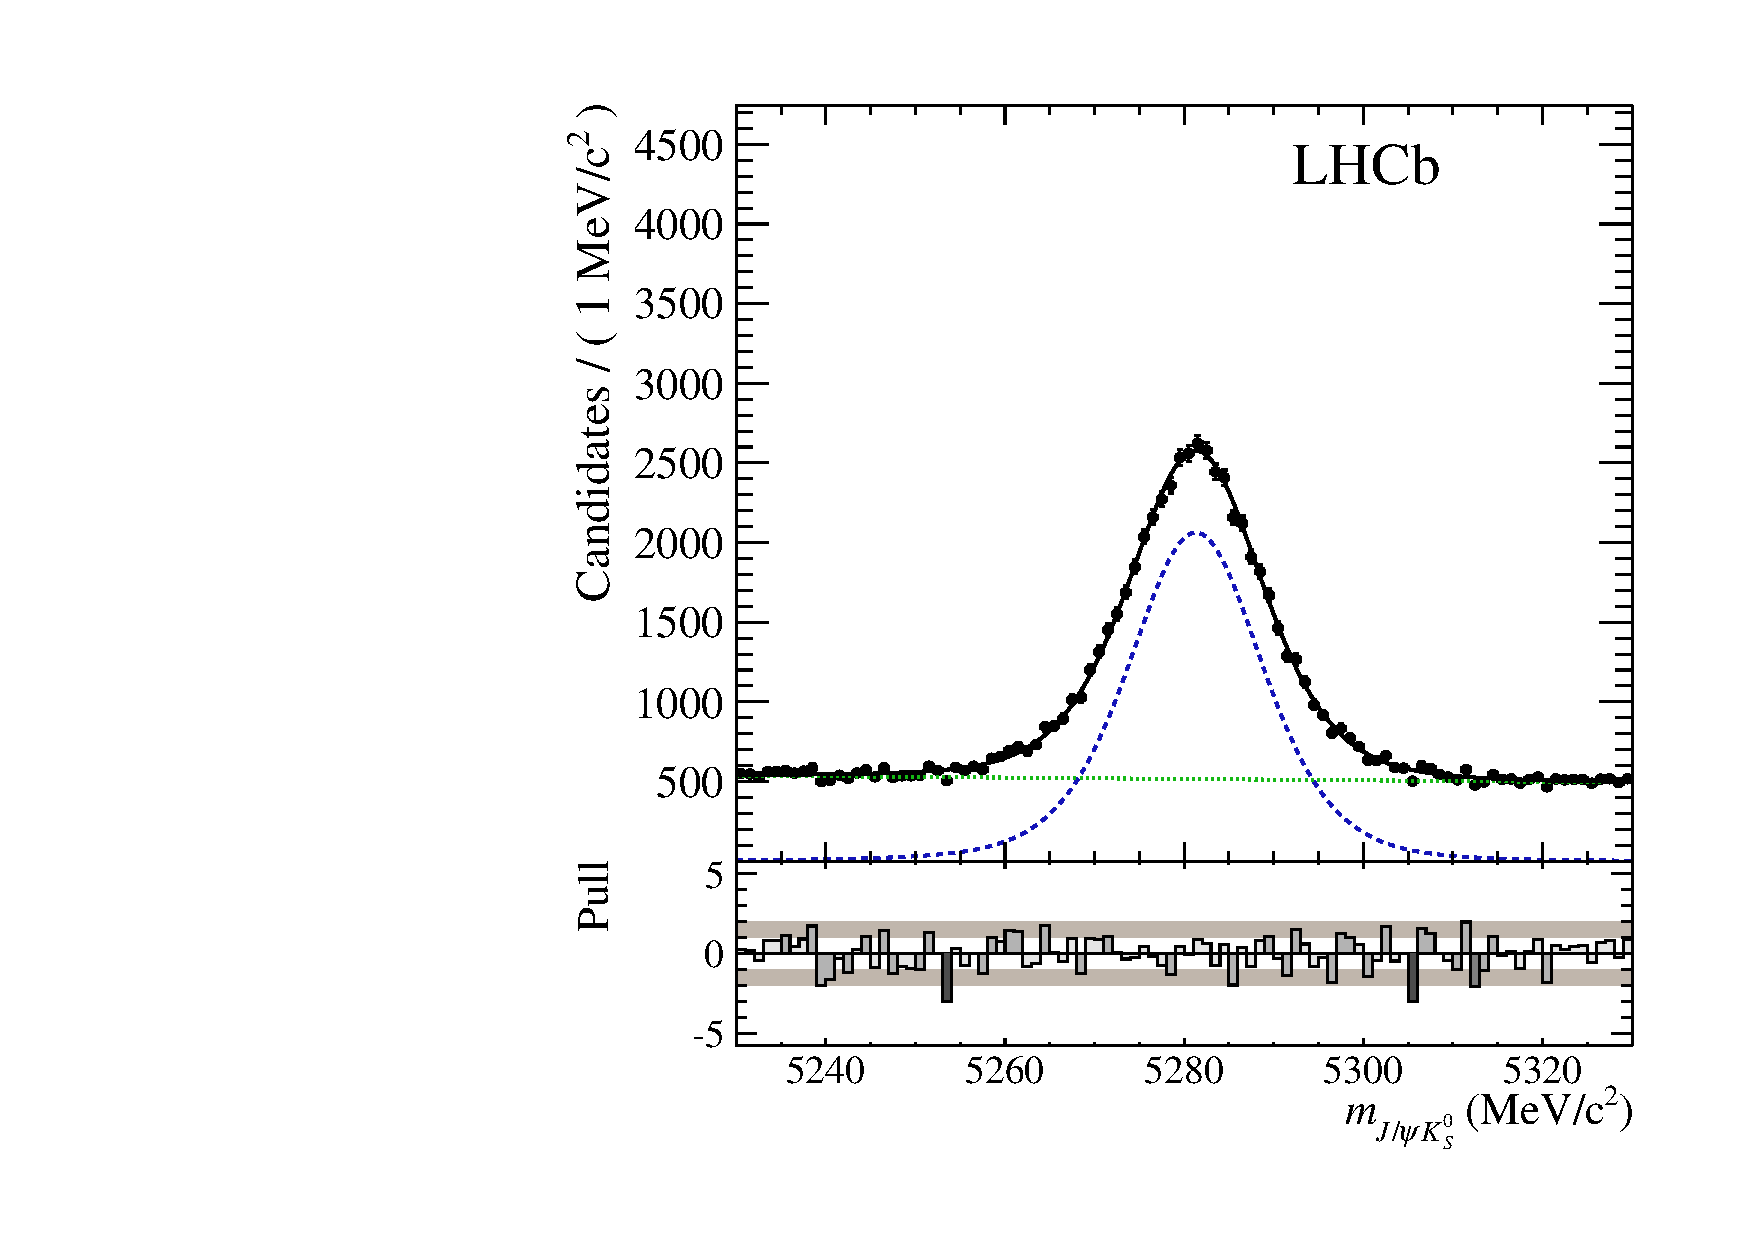
\includegraphics[width=0.4\textwidth]{private/content/measurement-of-sin2beta/figs/obsMass_summed_pull.pdf} 
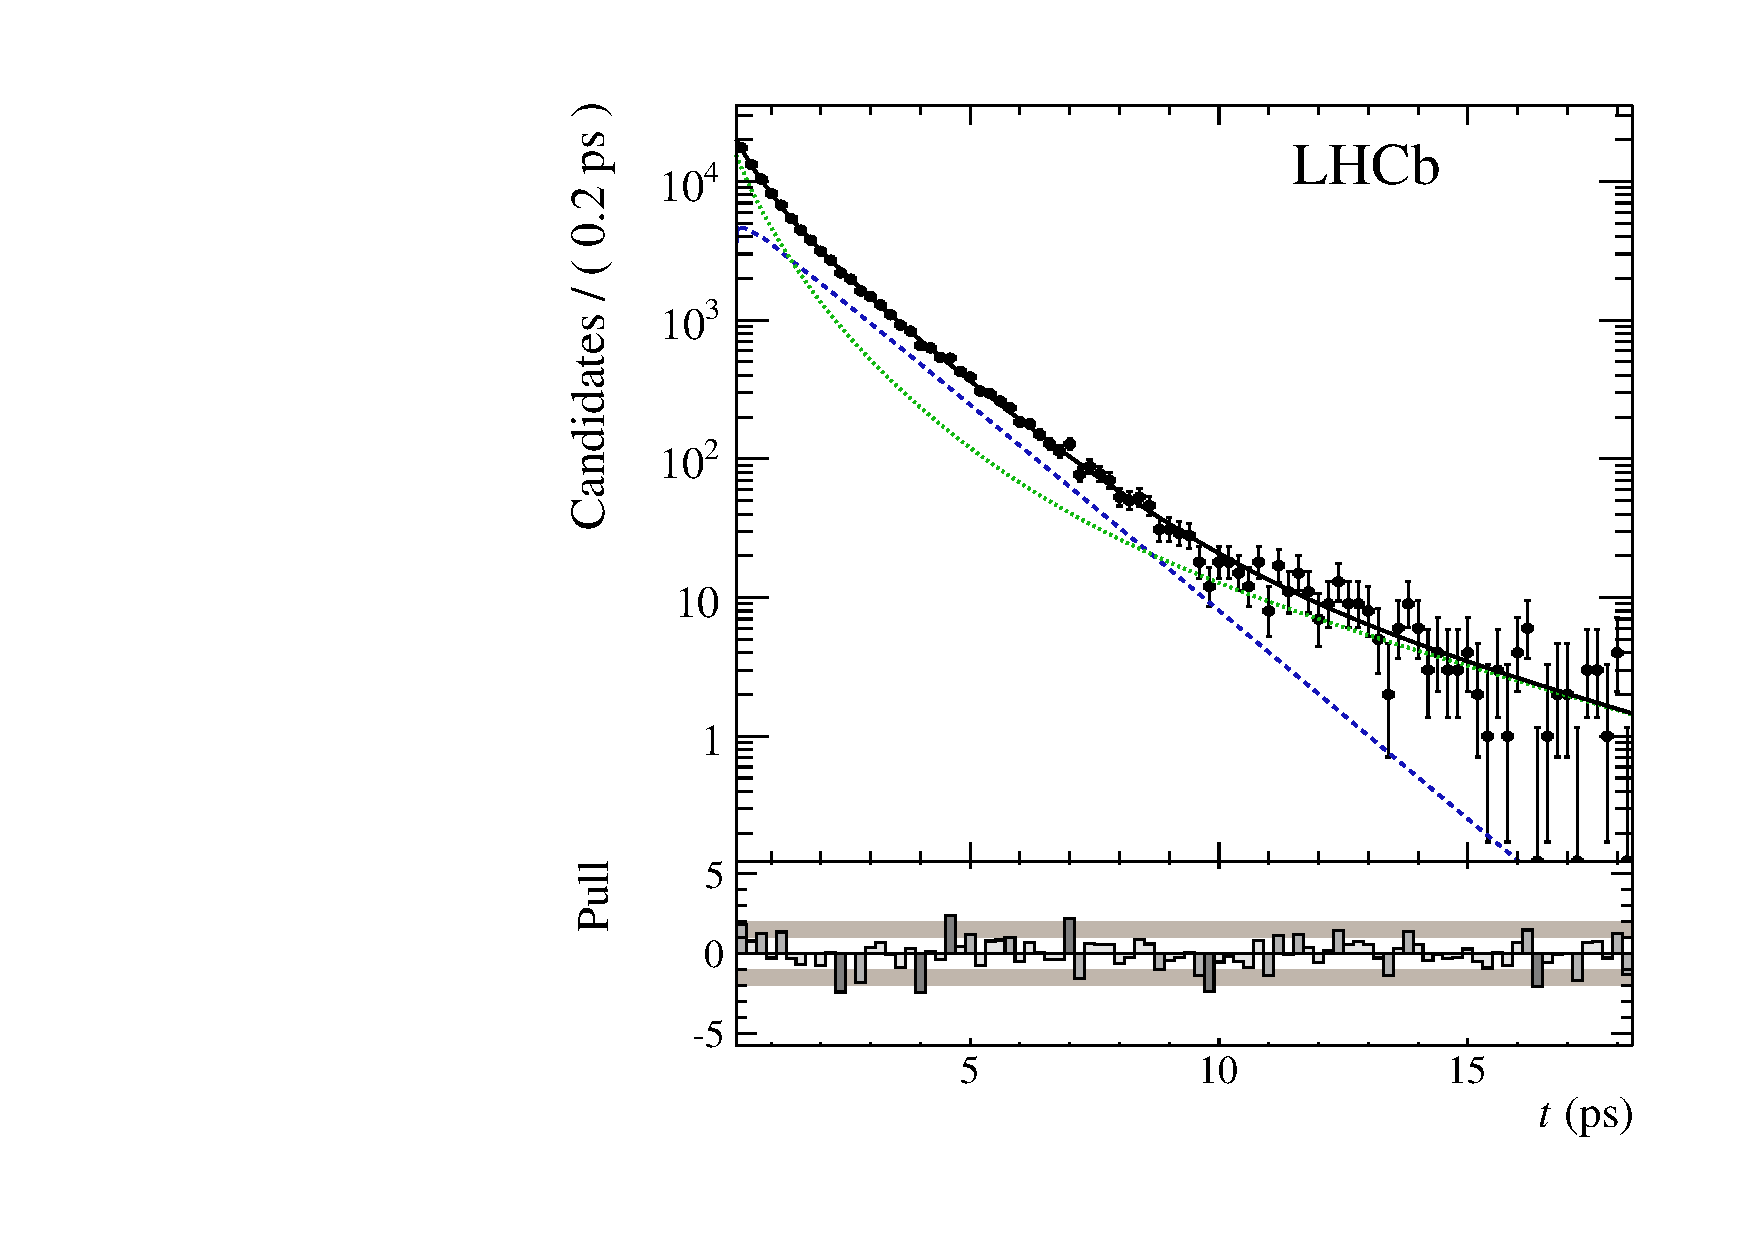
\includegraphics[width=0.4\textwidth]{private/content/measurement-of-sin2beta/figs/obsTime_summed_pull_log.pdf} \\
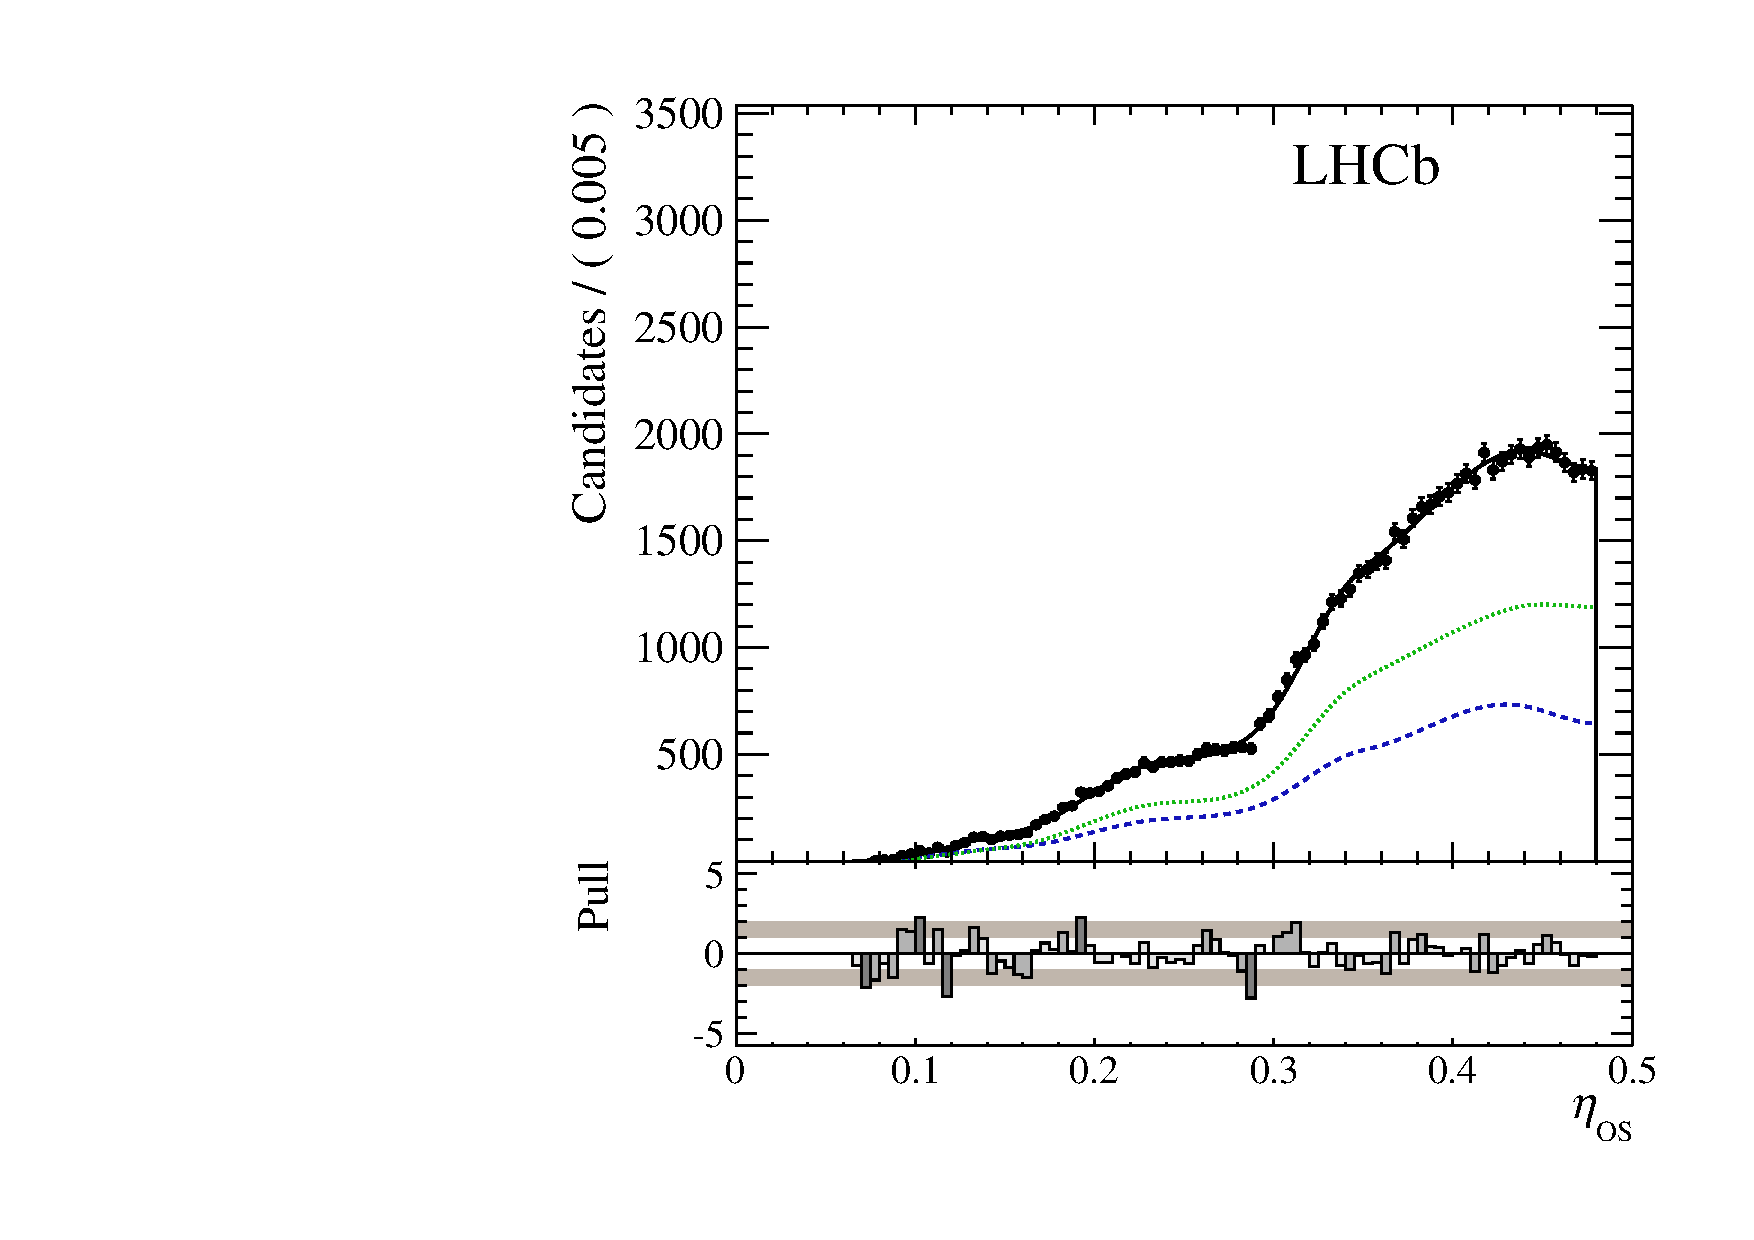
\includegraphics[width=0.4\textwidth]{private/content/measurement-of-sin2beta/figs/obsEtaOS_StdComb_CutOff_summed_pull.pdf}
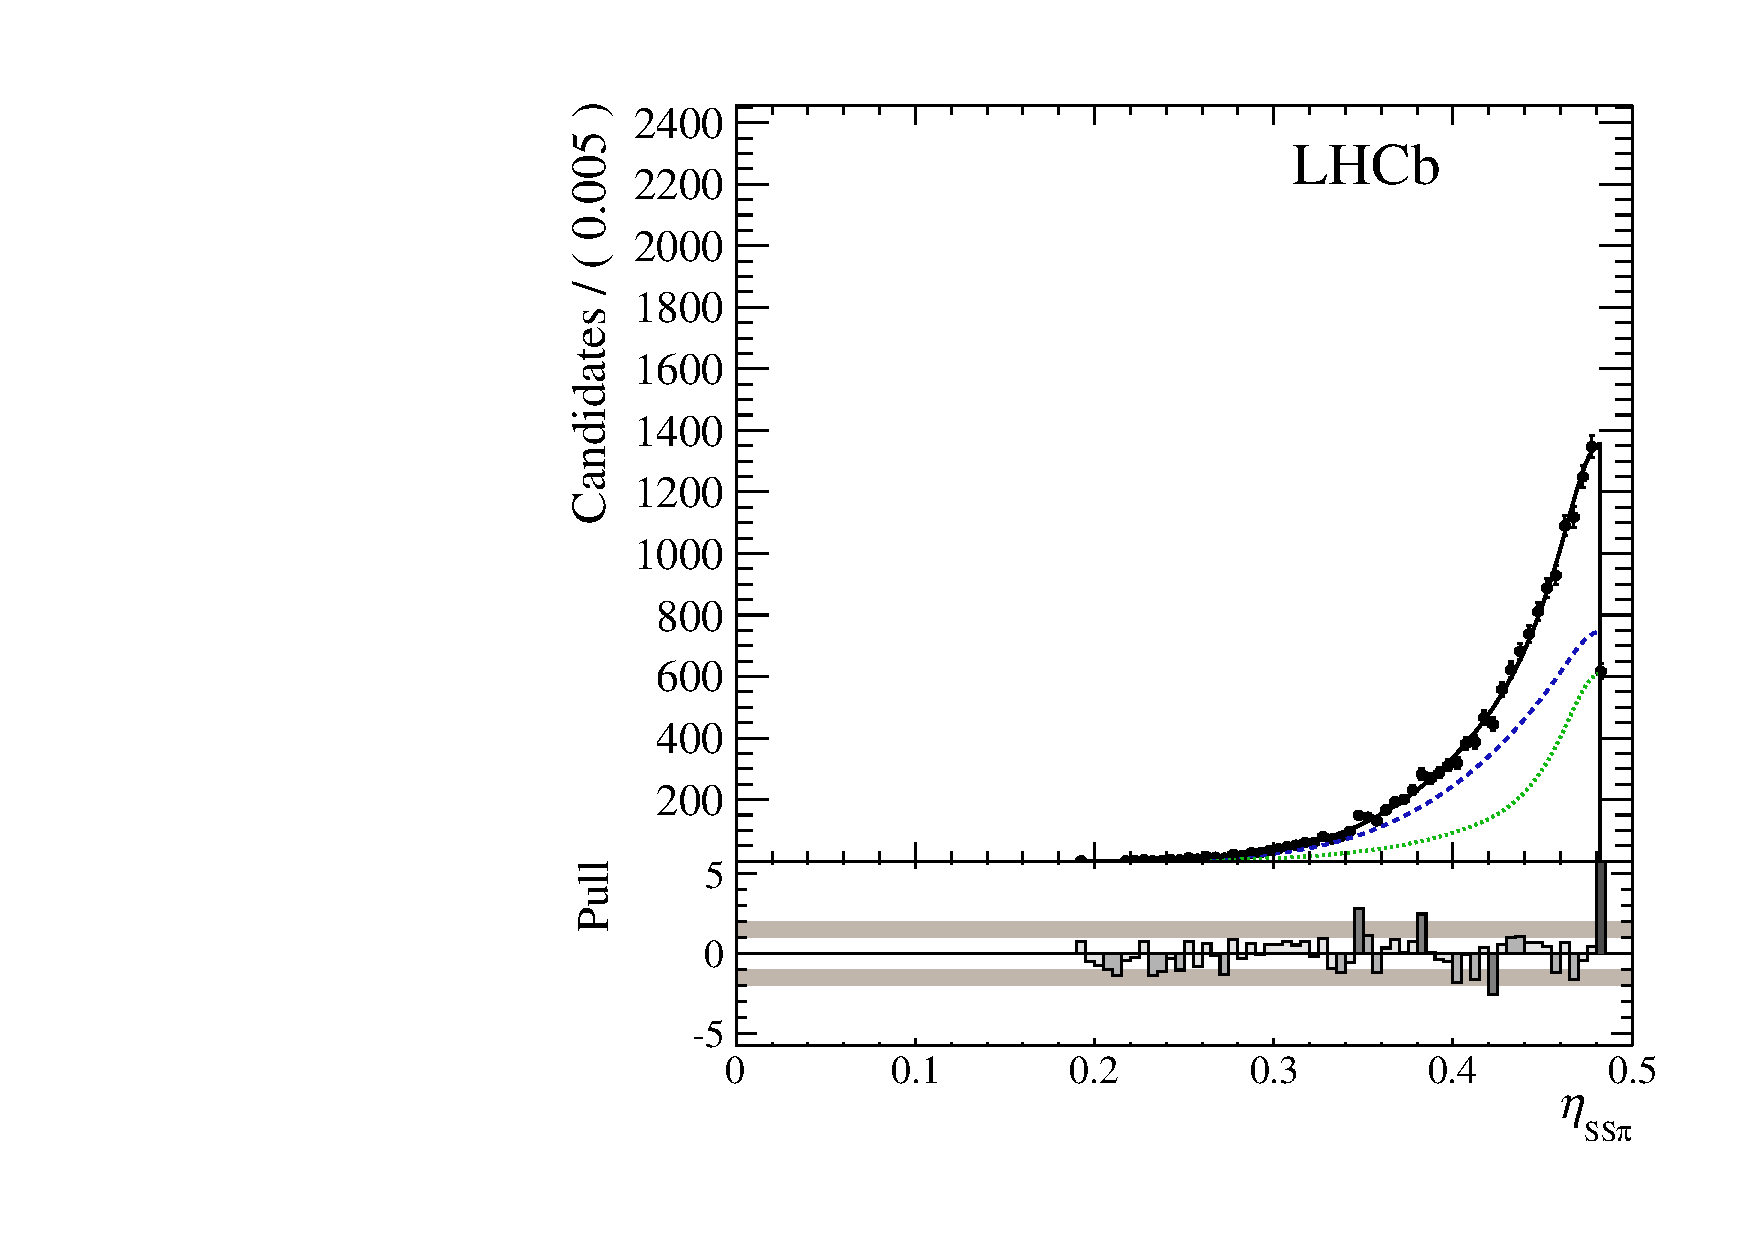
\includegraphics[width=0.4\textwidth]{private/content/measurement-of-sin2beta/figs/obsEtaSSPion_TupleCalib_summed_pull.pdf} \\
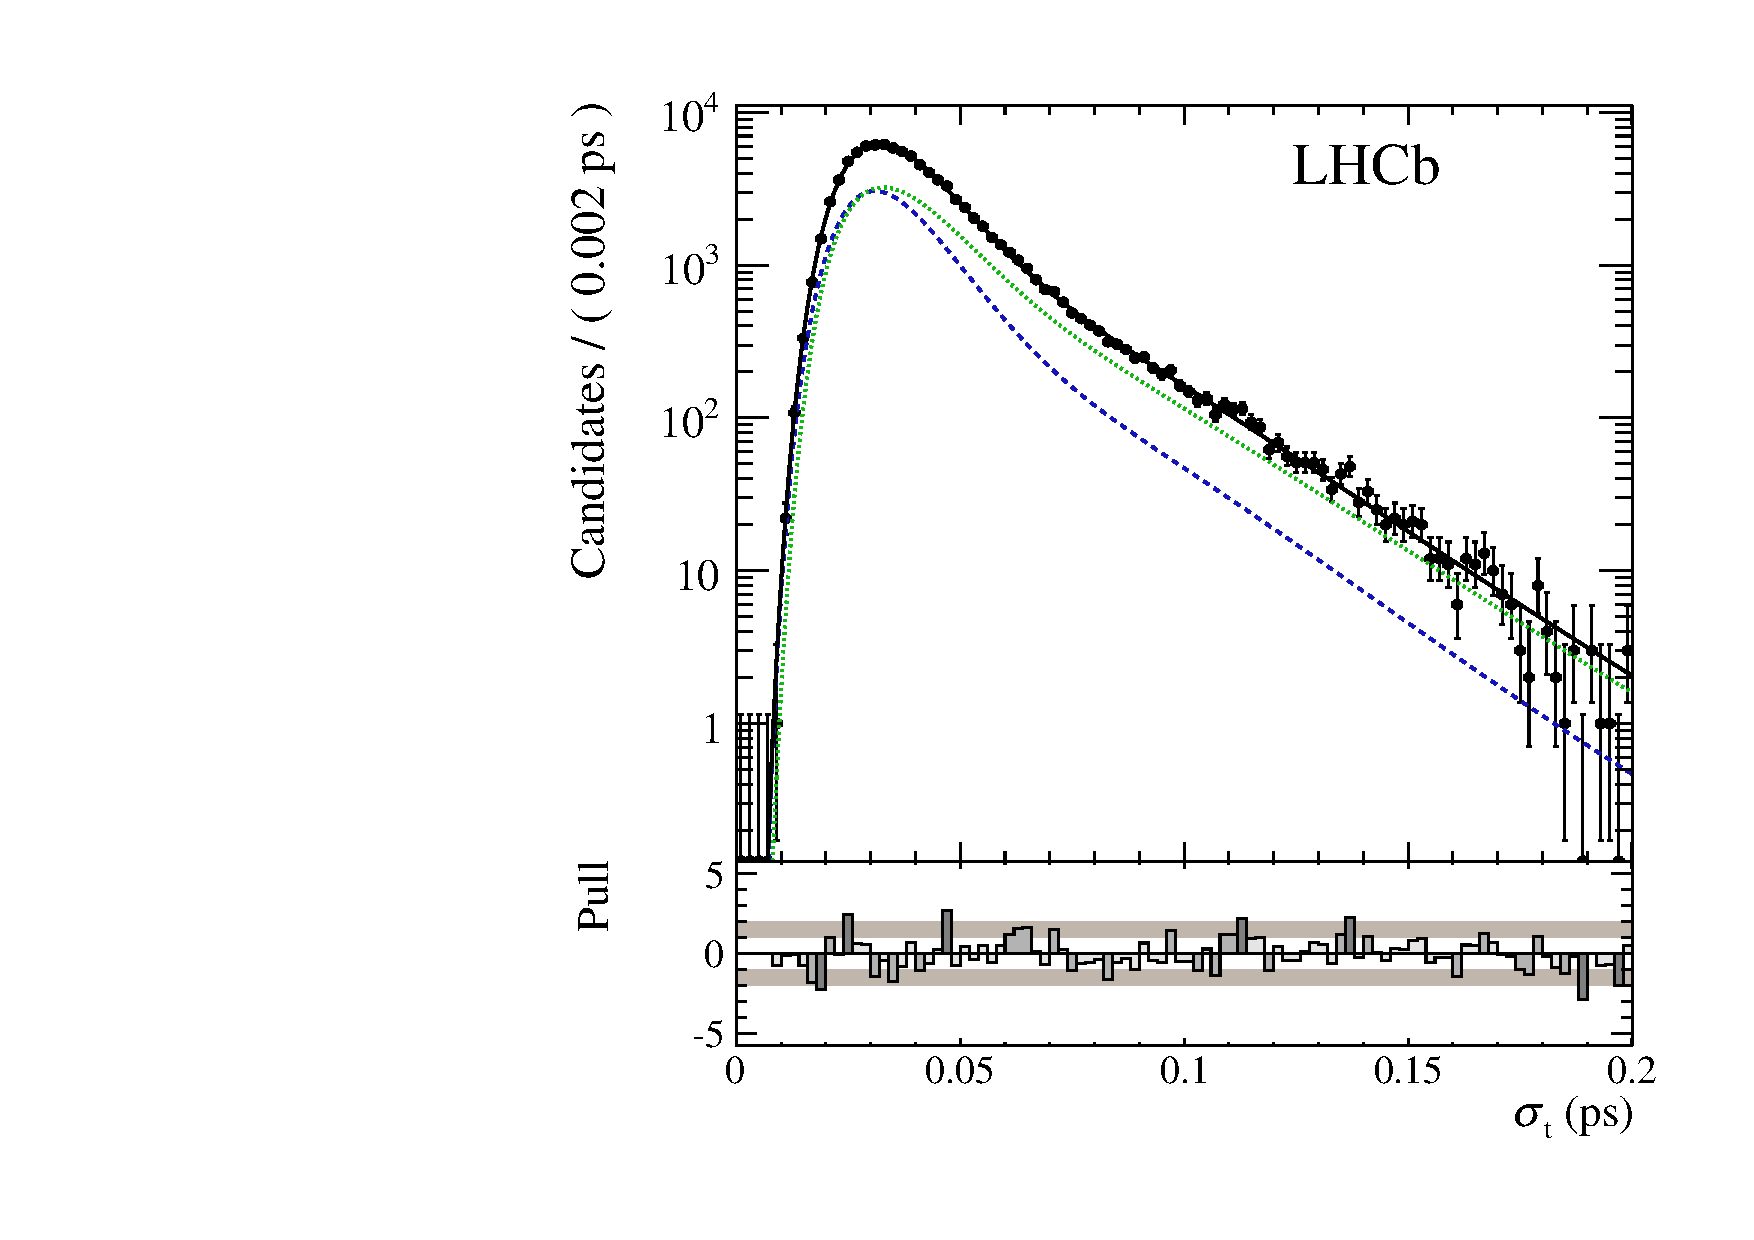
\includegraphics[width=0.4\textwidth]{private/content/measurement-of-sin2beta/figs/obsTimeError_summed_pull_log.pdf}
\caption{Plots of the \BdToJpsiKS data sample with the projected \PDF and pull
distributions. Shown is the reconstructed mass \obsMass (top left) and decay
time \obsTime (top right, logarithmic), per-event mistag (center; \obsEtaOS on
the left, \obsEtaSS on the right), and decay time error \obsTimeError (bottom,
logarithmic). Besides the data points and the full \PDF (solid black) the
projections of the signal (dashed blue) and the background (dotted green) are
shown.}
\label{fig:measurement_of_sin2beta:cpv_measurement:results:plots:dimensions}
\end{figure}

% ------------------------------------------------------------------------------
\subsection{Kaon regeneration}
\label{sec:measurement_of_sin2beta:cpv_measurement:kaon_regeneration}

\missing{Kaon regeneration}

